\documentclass{standalone}
\usepackage{tikz}
\usetikzlibrary{patterns, positioning}
\usepackage[sfdefault]{ClearSans} %% option 'sfdefault' activates Clear Sans as the default text font
\usepackage[T1]{fontenc}

\begin{document}
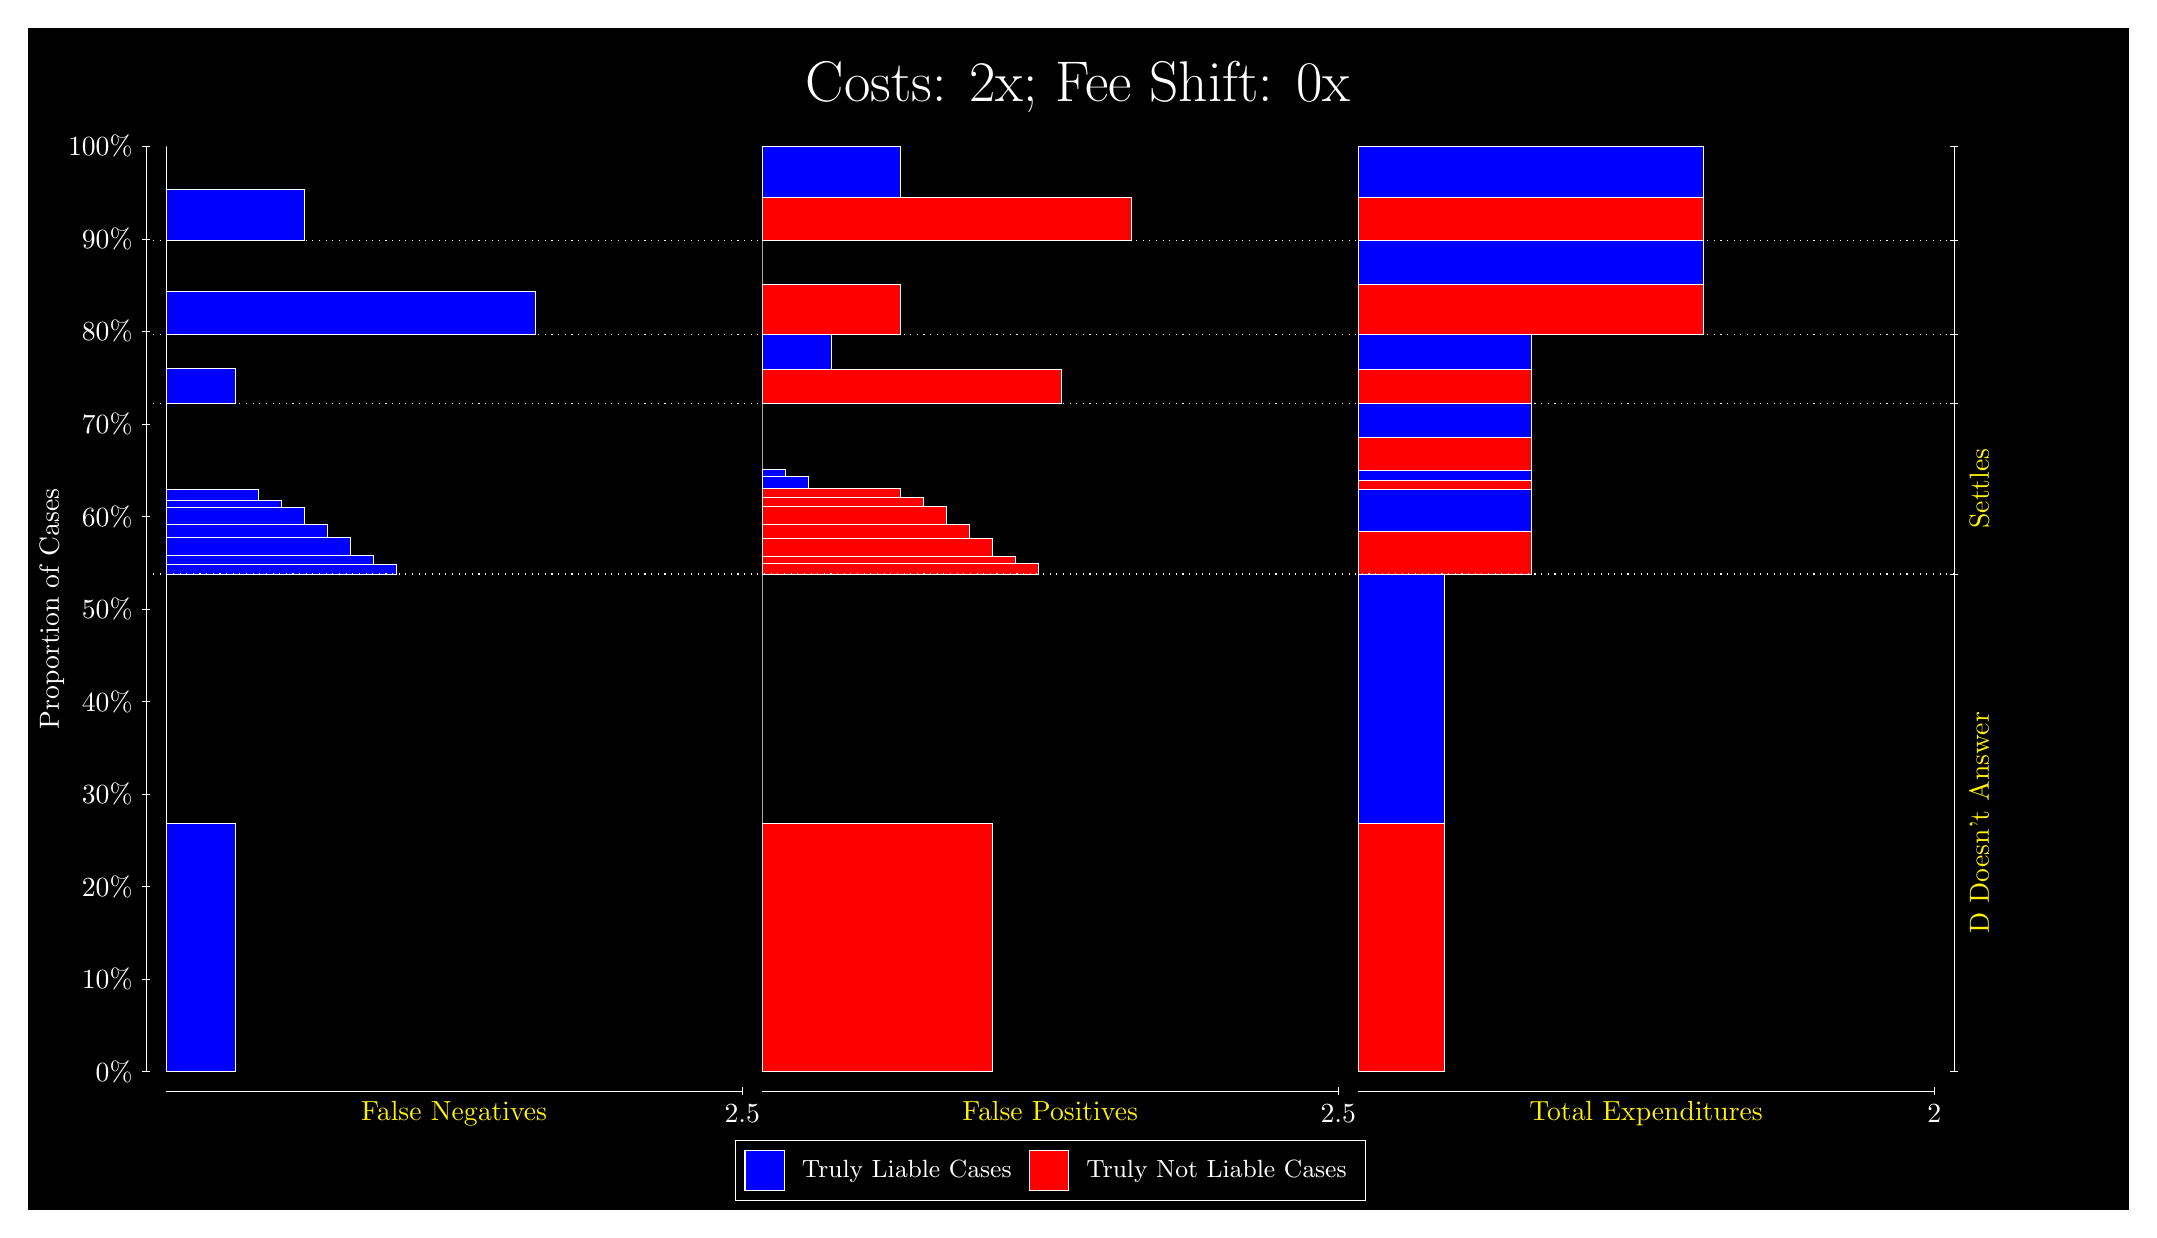
\begin{tikzpicture}
\draw[fill=black] (0,0) rectangle (26.667,15);
\draw[text=white] (0,13.5) rectangle (26.667,15) node[midway] {\huge Costs: 2x; Fee Shift: 0x};
\draw[white, very thin] (1.5,1.75) -- (1.5,13.5);
\node[rotate=90, text=white, anchor=center] at (0.3, 7.625) {Proportion of Cases};
\draw[white, very thin] (1.45,1.75) -- (1.55,1.75);
\node[text=white, anchor=east] at (1.45, 1.75) {0\%};
\draw[white, very thin] (1.45,2.925) -- (1.55,2.925);
\node[text=white, anchor=east] at (1.45, 2.925) {10\%};
\draw[white, very thin] (1.45,4.1) -- (1.55,4.1);
\node[text=white, anchor=east] at (1.45, 4.1) {20\%};
\draw[white, very thin] (1.45,5.275) -- (1.55,5.275);
\node[text=white, anchor=east] at (1.45, 5.275) {30\%};
\draw[white, very thin] (1.45,6.45) -- (1.55,6.45);
\node[text=white, anchor=east] at (1.45, 6.45) {40\%};
\draw[white, very thin] (1.45,7.625) -- (1.55,7.625);
\node[text=white, anchor=east] at (1.45, 7.625) {50\%};
\draw[white, very thin] (1.45,8.8) -- (1.55,8.8);
\node[text=white, anchor=east] at (1.45, 8.8) {60\%};
\draw[white, very thin] (1.45,9.975) -- (1.55,9.975);
\node[text=white, anchor=east] at (1.45, 9.975) {70\%};
\draw[white, very thin] (1.45,11.15) -- (1.55,11.15);
\node[text=white, anchor=east] at (1.45, 11.15) {80\%};
\draw[white, very thin] (1.45,12.325) -- (1.55,12.325);
\node[text=white, anchor=east] at (1.45, 12.325) {90\%};
\draw[white, very thin] (1.45,13.5) -- (1.55,13.5);
\node[text=white, anchor=east] at (1.45, 13.5) {100\%};

\draw[white, very thin] (24.457,1.75) -- (24.457,13.5);
\draw[white, very thin] (24.407,1.75) -- (24.507,1.75);
\node[anchor=west] at (24.407, 1.75) {};
\draw[white, very thin] (24.407,8.0679) -- (24.507,8.0679);
\node[anchor=west] at (24.407, 8.0679) {};
\draw[white, very thin] (24.407,10.239) -- (24.507,10.239);
\node[anchor=west] at (24.407, 10.239) {};
\draw[white, very thin] (24.407,11.112) -- (24.507,11.112);
\node[anchor=west] at (24.407, 11.112) {};
\draw[white, very thin] (24.407,12.305) -- (24.507,12.305);
\node[anchor=west] at (24.407, 12.305) {};
\draw[white, very thin] (24.407,13.5) -- (24.507,13.5);
\node[anchor=west] at (24.407, 13.5) {};

\draw[white, very thin, fill=blue] (1.75,1.75) rectangle (2.6283,4.9089);
\draw[white, very thin, fill=red] (1.75,4.9089) rectangle (1.75,8.0679);
\draw[white, very thin, fill=blue] (1.75,8.0679) rectangle (4.6775,8.1897);
\draw[white, very thin, fill=blue] (1.75,8.1897) rectangle (4.3848,8.306);
\draw[white, very thin, fill=blue] (1.75,8.306) rectangle (4.092,8.5305);
\draw[white, very thin, fill=blue] (1.75,8.5305) rectangle (3.7993,8.6993);
\draw[white, very thin, fill=blue] (1.75,8.6993) rectangle (3.5065,8.9132);
\draw[white, very thin, fill=blue] (1.75,8.9132) rectangle (3.2138,8.9998);
\draw[white, very thin, fill=blue] (1.75,8.9998) rectangle (2.921,9.1451);
\draw[white, very thin, fill=red] (1.75,9.1451) rectangle (1.75,10.239);
\draw[white, very thin, fill=blue] (1.75,10.239) rectangle (2.6283,10.678);
\draw[white, very thin, fill=red] (1.75,10.678) rectangle (1.75,11.112);
\draw[white, very thin, fill=blue] (1.75,11.112) rectangle (6.4341,11.663);
\draw[white, very thin, fill=red] (1.75,11.663) rectangle (1.75,12.305);
\draw[white, very thin, fill=blue] (1.75,12.305) rectangle (3.5065,12.954);
\draw[white, very thin, fill=red] (1.75,12.954) rectangle (1.75,13.5);
\draw[white, very thin, fill=red] (9.3189,1.75) rectangle (12.246,4.909);
\draw[white, very thin, fill=blue] (9.3189,4.909) rectangle (9.3189,8.0679);
\draw[white, very thin, fill=red] (9.3189,8.0679) rectangle (12.832,8.2048);
\draw[white, very thin, fill=red] (9.3189,8.2048) rectangle (12.539,8.2992);
\draw[white, very thin, fill=red] (9.3189,8.2992) rectangle (12.246,8.5272);
\draw[white, very thin, fill=red] (9.3189,8.5272) rectangle (11.954,8.6969);
\draw[white, very thin, fill=red] (9.3189,8.6969) rectangle (11.661,8.9225);
\draw[white, very thin, fill=red] (9.3189,8.9225) rectangle (11.368,9.0395);
\draw[white, very thin, fill=red] (9.3189,9.0395) rectangle (11.075,9.1619);
\draw[white, very thin, fill=blue] (9.3189,9.1619) rectangle (9.9044,9.3072);
\draw[white, very thin, fill=blue] (9.3189,9.3072) rectangle (9.6116,9.3938);
\draw[white, very thin, fill=blue] (9.3189,9.3938) rectangle (9.3189,10.239);
\draw[white, very thin, fill=red] (9.3189,10.239) rectangle (13.125,10.674);
\draw[white, very thin, fill=blue] (9.3189,10.674) rectangle (10.197,11.112);
\draw[white, very thin, fill=red] (9.3189,11.112) rectangle (11.075,11.754);
\draw[white, very thin, fill=blue] (9.3189,11.754) rectangle (9.3189,12.305);
\draw[white, very thin, fill=red] (9.3189,12.305) rectangle (14.003,12.851);
\draw[white, very thin, fill=blue] (9.3189,12.851) rectangle (11.075,13.5);
\draw[white, very thin, fill=red] (16.888,1.75) rectangle (17.986,4.909);
\draw[white, very thin, fill=blue] (16.888,4.909) rectangle (17.986,8.0679);
\draw[white, very thin, fill=red] (16.888,8.0679) rectangle (19.083,8.6159);
\draw[white, very thin, fill=blue] (16.888,8.6159) rectangle (19.083,9.1409);
\draw[white, very thin, fill=red] (16.888,9.1409) rectangle (19.083,9.2633);
\draw[white, very thin, fill=blue] (16.888,9.2633) rectangle (19.083,9.385);
\draw[white, very thin, fill=red] (16.888,9.385) rectangle (19.083,9.8086);
\draw[white, very thin, fill=blue] (16.888,9.8086) rectangle (19.083,10.239);
\draw[white, very thin, fill=red] (16.888,10.239) rectangle (19.083,10.674);
\draw[white, very thin, fill=blue] (16.888,10.674) rectangle (19.083,11.112);
\draw[white, very thin, fill=red] (16.888,11.112) rectangle (21.279,11.754);
\draw[white, very thin, fill=blue] (16.888,11.754) rectangle (21.279,12.305);
\draw[white, very thin, fill=red] (16.888,12.305) rectangle (21.279,12.851);
\draw[white, very thin, fill=blue] (16.888,12.851) rectangle (21.279,13.5);
\draw[white, dotted] (1.5,8.0679) -- (24.457,8.0679);
\draw[white, dotted] (1.5,10.239) -- (24.457,10.239);
\draw[white, dotted] (1.5,11.112) -- (24.457,11.112);
\draw[white, dotted] (1.5,12.305) -- (24.457,12.305);
\draw[white, very thin] (1.75,1.5) -- (9.0689,1.5);
\node[text=yellow, anchor=north] at (5.4094, 1.5) {False Negatives};
\draw[white, very thin] (9.0689,1.45) -- (9.0689,1.55);
\node[text=white, anchor=north] at (9.0689, 1.45) {2.5};

\draw[white, very thin] (9.3189,1.5) -- (16.638,1.5);
\node[text=yellow, anchor=north] at (12.978, 1.5) {False Positives};
\draw[white, very thin] (16.638,1.45) -- (16.638,1.55);
\node[text=white, anchor=north] at (16.638, 1.45) {2.5};

\draw[white, very thin] (16.888,1.5) -- (24.207,1.5);
\node[text=yellow, anchor=north] at (20.547, 1.5) {Total Expenditures};
\draw[white, very thin] (24.207,1.45) -- (24.207,1.55);
\node[text=white, anchor=north] at (24.207, 1.45) {2};

\node[text=yellow, centered, rotate=90] at (24.777, 4.9089) {D Doesn't Answer};
\node[text=yellow, centered, rotate=90] at (24.777, 9.1535) {Settles};




\draw (12.978300999999998,1.5) node[draw=none] (baseCoordinate) {};
\begin{scope}[align=center]
        \matrix[scale=0.5, draw=white, below=0.5cm of baseCoordinate, nodes={draw}, column sep=0.1cm]{
            \node[rectangle, draw, minimum width=0.5cm, minimum height=0.5cm, fill=blue] {}; &
            \node[draw=none, font=\small, text=white] (B) {Truly Liable Cases}; &
            \node[rectangle, draw, minimum width=0.5cm, minimum height=0.5cm, fill=red] {}; &
            \node[draw=none, font=\small, text=white] (B) {Truly Not Liable Cases}; \\
            };
\end{scope}

\end{tikzpicture}
\end{document}